\section{定点数与浮点数}\label{sec:NumberSystemBasics/fixed-point-and-floating-point}
    解决了整数的记录问题之后,我们需要考虑小数的记录的问题。

    \subsection{定点数}\label{subsec:NumberSystemBasics/fixed-point-and-floating-point/fixed-point}

        我们可以参考之前学到的方式,直接记录小数的二进制。由于二进制中可用的数码 $0$ 和 $1$ 已经被全部用于表达数,因此已经没有记号用于在数码间标记小数点位置并且不造成歧义,所以需要人为预先规定小数点的位置。假设左起第一位为符号位,然后假设把小数点定在 $n$ 位与 $n + 1$ 位之间,剩下的为小数部分的话,那么可以表达的数的范围为 $(-\underbrace{11 \cdots 11}_{n-1}.\underbrace{11 \cdots 11}_{k-n})_2$ -- $(-0.\underbrace{00 \cdots 00}_{k-n}1)_2$ 和 $(0.\underbrace{00 \cdots 00}_{k-n}1)_2$ -- $(\underbrace{11 \cdots 11}_{n-1}.\underbrace{11 \cdots 11}_{k-n})_2$,分度值为 $(0.\underbrace{00 \cdots 00}_{k-n}1)_2$,或者转为十进制是 $-\frac{2^{(k-1)}-1}{2^{(k-n)}}$ -- $-\frac{1}{2^{(k-n)}}$ 和 $\frac{1}{2^{(k-n)}}$ -- $\frac{2^{(k-1)}-1}{2^{(k-n)}}$,分度值为 $\frac{1}{2^{(k-n)}}$。

        一个具体的例子如~\ref{fig:NumberSystemBasics/fixed-point-and-floating-point/fixed-point/data-range} 所示。

        % https://tex.stackexchange.com/a/130008/149813
        \begin{figure}
            \centering
            \begin{tabular}{lS[table-format=-3.7]S[table-format=-3.7]S[table-format=-3.7]}
                $n$ & 最小值     & 最大值    & 分度值    \\ \hline
                1   & -0.9921875 & 0.9921875  & 0.0078125 \\
                2   & -1.984375  & 1.984375   & 0.015625  \\
                3   & -3.96875   & 3.96875    & 0.03125   \\
                4   & -7.9375    & 7.9375     & 0.0625    \\
                5   & -15.875    & 15.875     & 0.125     \\
                6   & -31.75     & 31.75      & 0.25      \\
                7   & -63.5      & 63.5       & 0.5       \\
                8   & -127       & 127        & 1         \\
            \end{tabular}
            \caption{$k = 8$ 时 $n$ 的值对应的数据范围}
            \label{fig:NumberSystemBasics/fixed-point-and-floating-point/fixed-point/data-range}
        \end{figure}

        这种记录小数的方式,其小数点的位置是固定的,因此被称为定点数(Fixed Point)。比如说,对于二进制小数 $(101.01)_2$ 来说,在不损耗精度的前提下,不管如何修改上面的定义中的参数(即 $k$ 与 $n$),记录的小数点总是会在第二个 $1$ 和 $0$ 之间,这个小数点相对于这个数的位置是固定不变的,这就是“定点数”名称的来源。

        然而,这种记录方式有一个问题,就是无法在精度和范围中间达到平衡:如果采用更小的 $n$,那么可以提高精度,但是可以表达的数的范围便急剧减小;而如果试图提高范围,那么就得采用更大的 $n$,此时精度便开始降低。这个我们没有让“数码在数字中的位置”这个信息灵活起来。如果我们将存储所使用的权重在对数数轴上标记的话,那么会是如图~\ref{fig:NumberSystemBasics/fixed-point-and-floating-point/fixed-point/position} 所示的情况:

        \begin{figure}
            \centering
            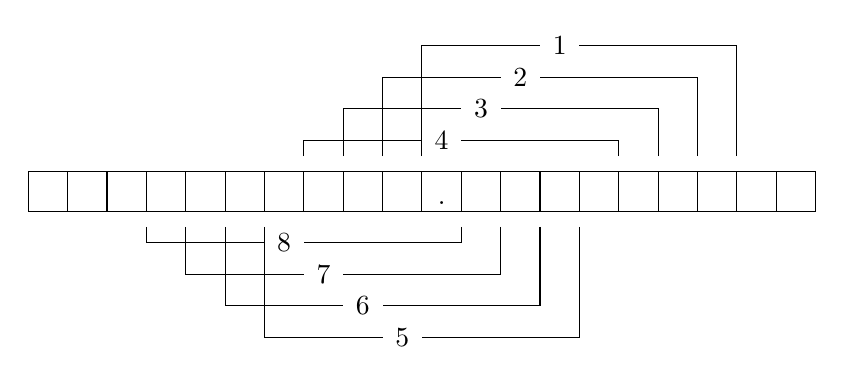
\begin{tikzpicture}
                \draw [step = 0.5] (0, 0) grid (10, 0.5);
                \node at (5.25, 0.1) {.};

                \draw (1.5, -0.2) -- (1.5, -0.4) -- (3, -0.4);
                \draw (5.5, -0.2) -- (5.5, -0.4) -- (3.5, -0.4);
                \node at (3.25, -0.4) {8};

                \draw (2, -0.2) -- (2, -0.8) -- (3.5, -0.8);
                \draw (6, -0.2) -- (6, -0.8) -- (4, -0.8);
                \node at (3.75, -0.8) {7};

                \draw (2.5, -0.2) -- (2.5, -1.2) -- (4, -1.2);
                \draw (6.5, -0.2) -- (6.5, -1.2) -- (4.5, -1.2);
                \node at (4.25, -1.2) {6};

                \draw (3, -0.2) -- (3, -1.6) -- (4.5, -1.6);
                \draw (7, -0.2) -- (7, -1.6) -- (5, -1.6);
                \node at (4.75, -1.6) {5};

                \draw (3.5, 0.7) -- (3.5, 0.9) -- (5, 0.9);
                \draw (7.5, 0.7) -- (7.5, 0.9) -- (5.5, 0.9);
                \node at (5.25, 0.9) {4};

                \draw (4, 0.7) -- (4, 1.3) -- (5.5, 1.3);
                \draw (8, 0.7) -- (8, 1.3) -- (6, 1.3);
                \node at (5.75, 1.3) {3};

                \draw (4.5, 0.7) -- (4.5, 1.7) -- (6, 1.7);
                \draw (8.5, 0.7) -- (8.5, 1.7) -- (6.5, 1.7);
                \node at (6.25, 1.7) {2};

                \draw (5, 0.7) -- (5, 2.1) -- (6.5, 2.1);
                \draw (9, 0.7) -- (9, 2.1) -- (7, 2.1);
                \node at (6.75, 2.1) {1};
            \end{tikzpicture}
            \caption{存储位在数轴上的位置}
            \label{fig:NumberSystemBasics/fixed-point-and-floating-point/fixed-point/position}
        \end{figure}

    \subsection{浮点数}\label{subsec:NumberSystemBasics/fixed-point-and-floating-point/floating-point}
        回想一下,当我们遇到一个比较大或者比较小的数的时候,我们通常使用科学记数法(Scientific Notation)来简化记录。为了取得精度和范围的平衡,我们可以借鉴科学记数法,使用一定的存储位表达“位置”,用余下的存储位来存储数值。诚然,在有限的存储位中再抠出一部分用于存储“位置”会损失精度,但是我们换来了更大的数值范围,而且对于大一点的数字而言,只要我们充分地权衡好这个损失的量,那么损失少量的精度是可以接受的。
